\documentclass{book}
\usepackage[utf8]{vietnam}
\usepackage{cite}
\usepackage{amsmath,amssymb,amsfonts}
\usepackage{algorithm}
\usepackage{algorithmic}
\usepackage{graphicx}
\usepackage{textcomp}
\usepackage{xcolor}
\usepackage{tabularx}
\usepackage{listings}
\usepackage{enumerate}

\newcounter{savedenum}
\newcommand*{\saveenum}{\setcounter{savedenum}{\theenumi}}
\newcommand*{\resume}{\setcounter{enumi}{\thesavedenum}}


\begin{document}
%\title{TỐI ƯU LỒI VÀ ỨNG DỤNG TRONG MÁY HỌC}
%\author{Võ Thị Lưu Phương}
%
%
%\maketitle


\setcounter{chapter}{1}
\chapter{HÀM LỒI}
\textit{Tác giả: Võ Thị Lưu Phương\\Email: vtlphuong@hcmiu.edu.vn}


\section{Tập lồi}
Tập $C$ trong không gian bấy kỳ được gọi là lồi nếu và chỉ nếu cho bất kỳ hai điểm $x_1, x_2 \in C$ và số thực $\theta \in [0,1]$, điểm $\theta x_1 + (1-\theta) x_2$ cũng thuộc $C$ (xem Hình \ref{fig:convexset}).

Định nghĩa có thể được mở rộng ra cho $n$ điểm $x_1, \ldots, x_n \in C$. 
Tập $C$ là lồi nếu và chỉ nếu $\theta_1 x_1 + \ldots + \theta_n x_n \in C$ với bất kỳ $n$ số thực $\theta_1, \ldots, \theta_n \in [0,1]$, $\theta_1 + \ldots + \theta_n = 1$.
\begin{figure}[h]
	\centering
	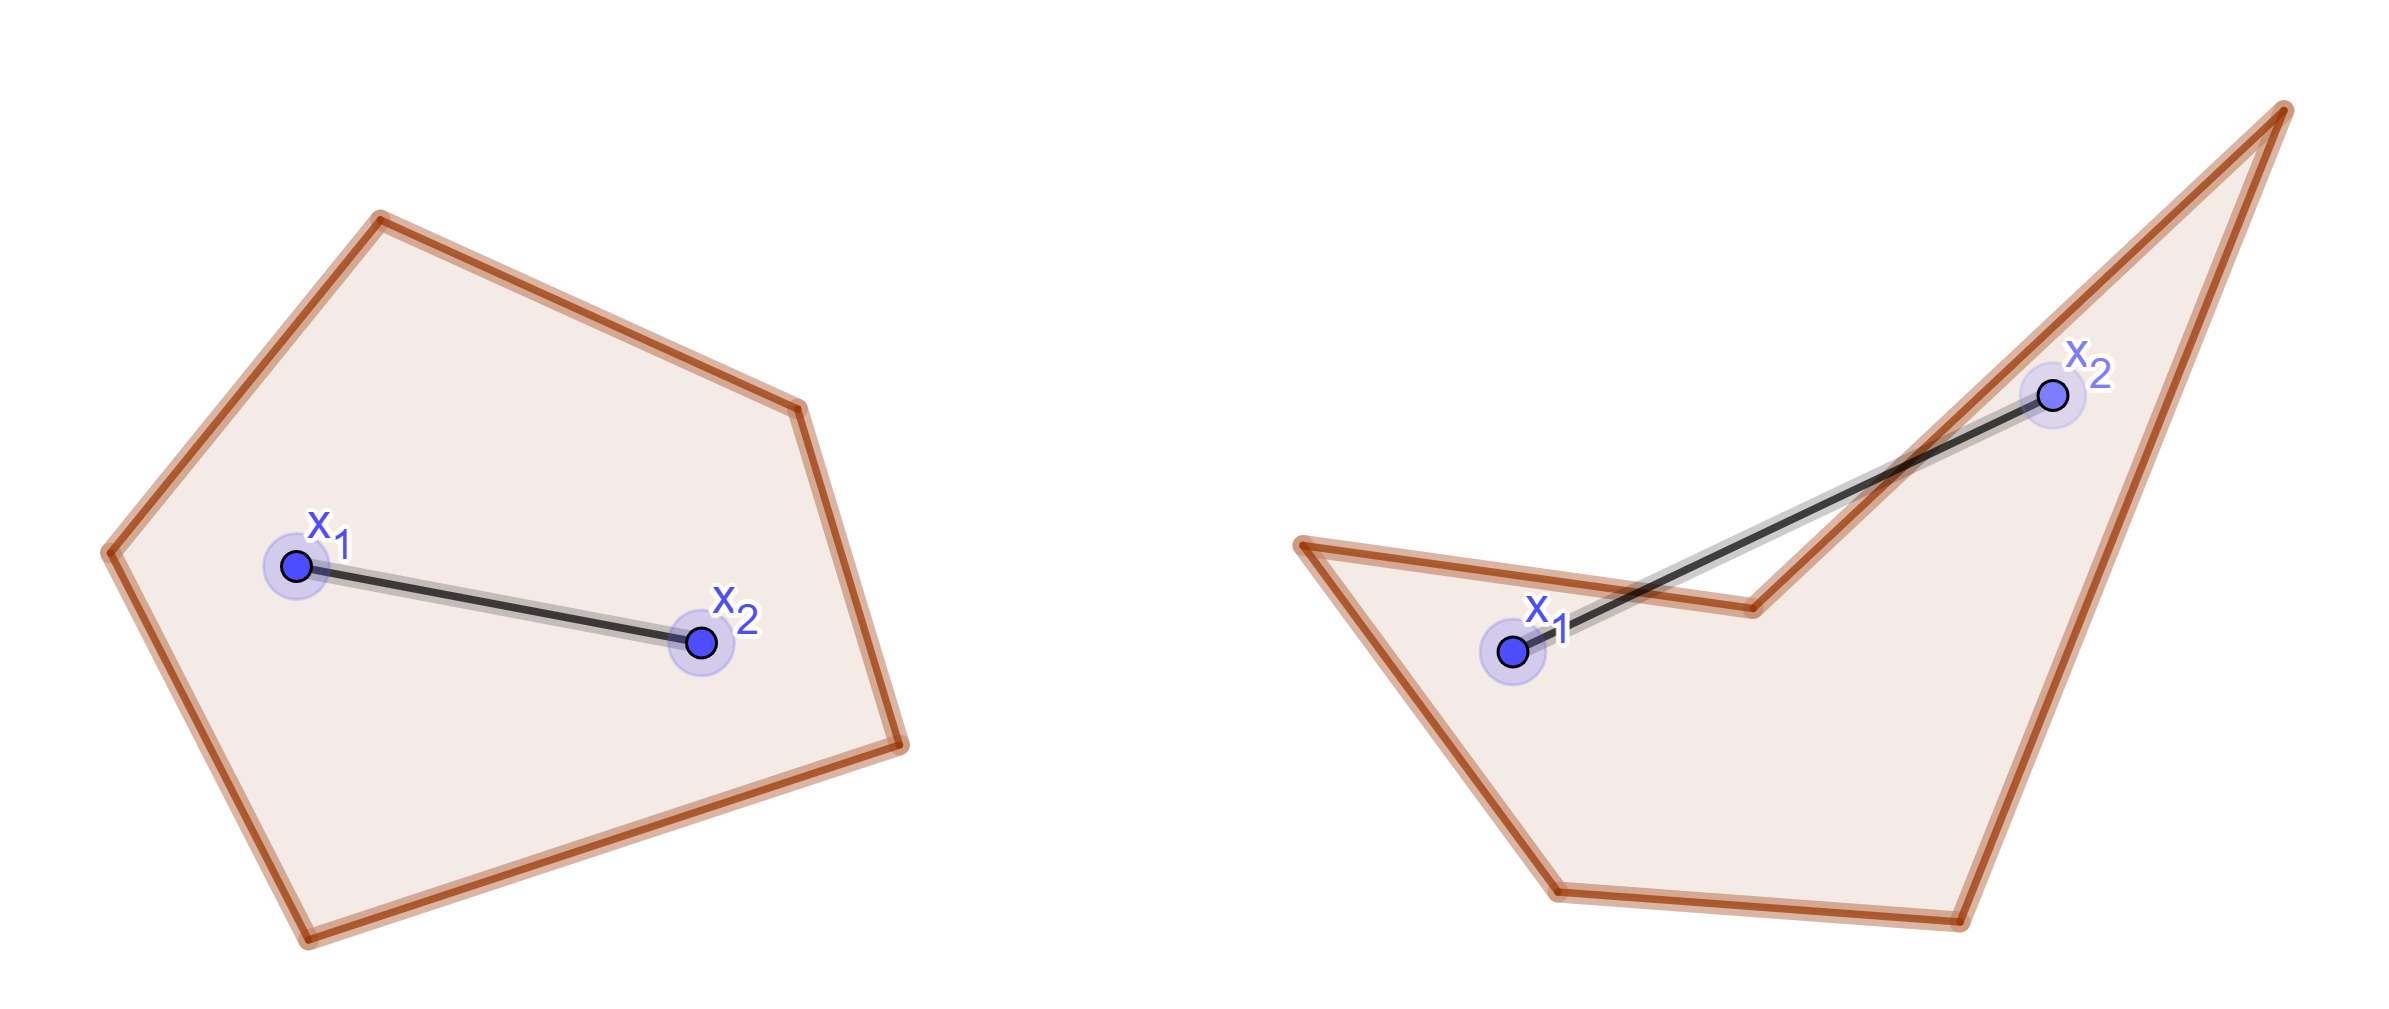
\includegraphics[width=9.5cm]{hinh_chuong2_convexfunc/chap2_convex-noncovex-set_v2.png}
	\caption{Hình mình họa tập lồi (trái) và tập không lồi (phải) trong không gian 2D.}
	\label{fig:convexset}	
\end{figure}

Lưu ý, điểm $\theta x_1 + (1-\theta) x_2$ được gọi là \textit{kết hợp tuyến tính} (linear combination) của hai điểm $x_1$ và $x_2$. trong mặt phẳng 2D điểm $\theta x_1 + (1-\theta) x_2$ là một điểm nằm trong đoạn thẳng nối hai điểm $x_1$ và $x_2$. Khi $\theta$ biến thiên từ 0 đến 1, tập các điểm $\theta x_1 + (1-\theta) x_2$ cũng chính là đoạn thẳng nối $x_1$ và $x_2$ với $\theta = 0$ chính là điểm $x_2$ và $\theta=1$ là điểm $x_1$.
Khi mở rộng khái niệm trên cho nhiều điểm $x_1, \ldots, x_n$ thì ta có khái niệm convex hull, tập hợp các điểm là kết hợp tuyến tính của $n$ điểm $x_1, \ldots, x_n$:
\begin{align*}
\rm{conv} C = \{\theta_1 x_1 + \ldots + \theta_n x_n, \forall \theta_i \geq 0, \theta_1+\ldots+\theta_n = 1\}.
\end{align*}
\begin{figure}[h]
	\centering
	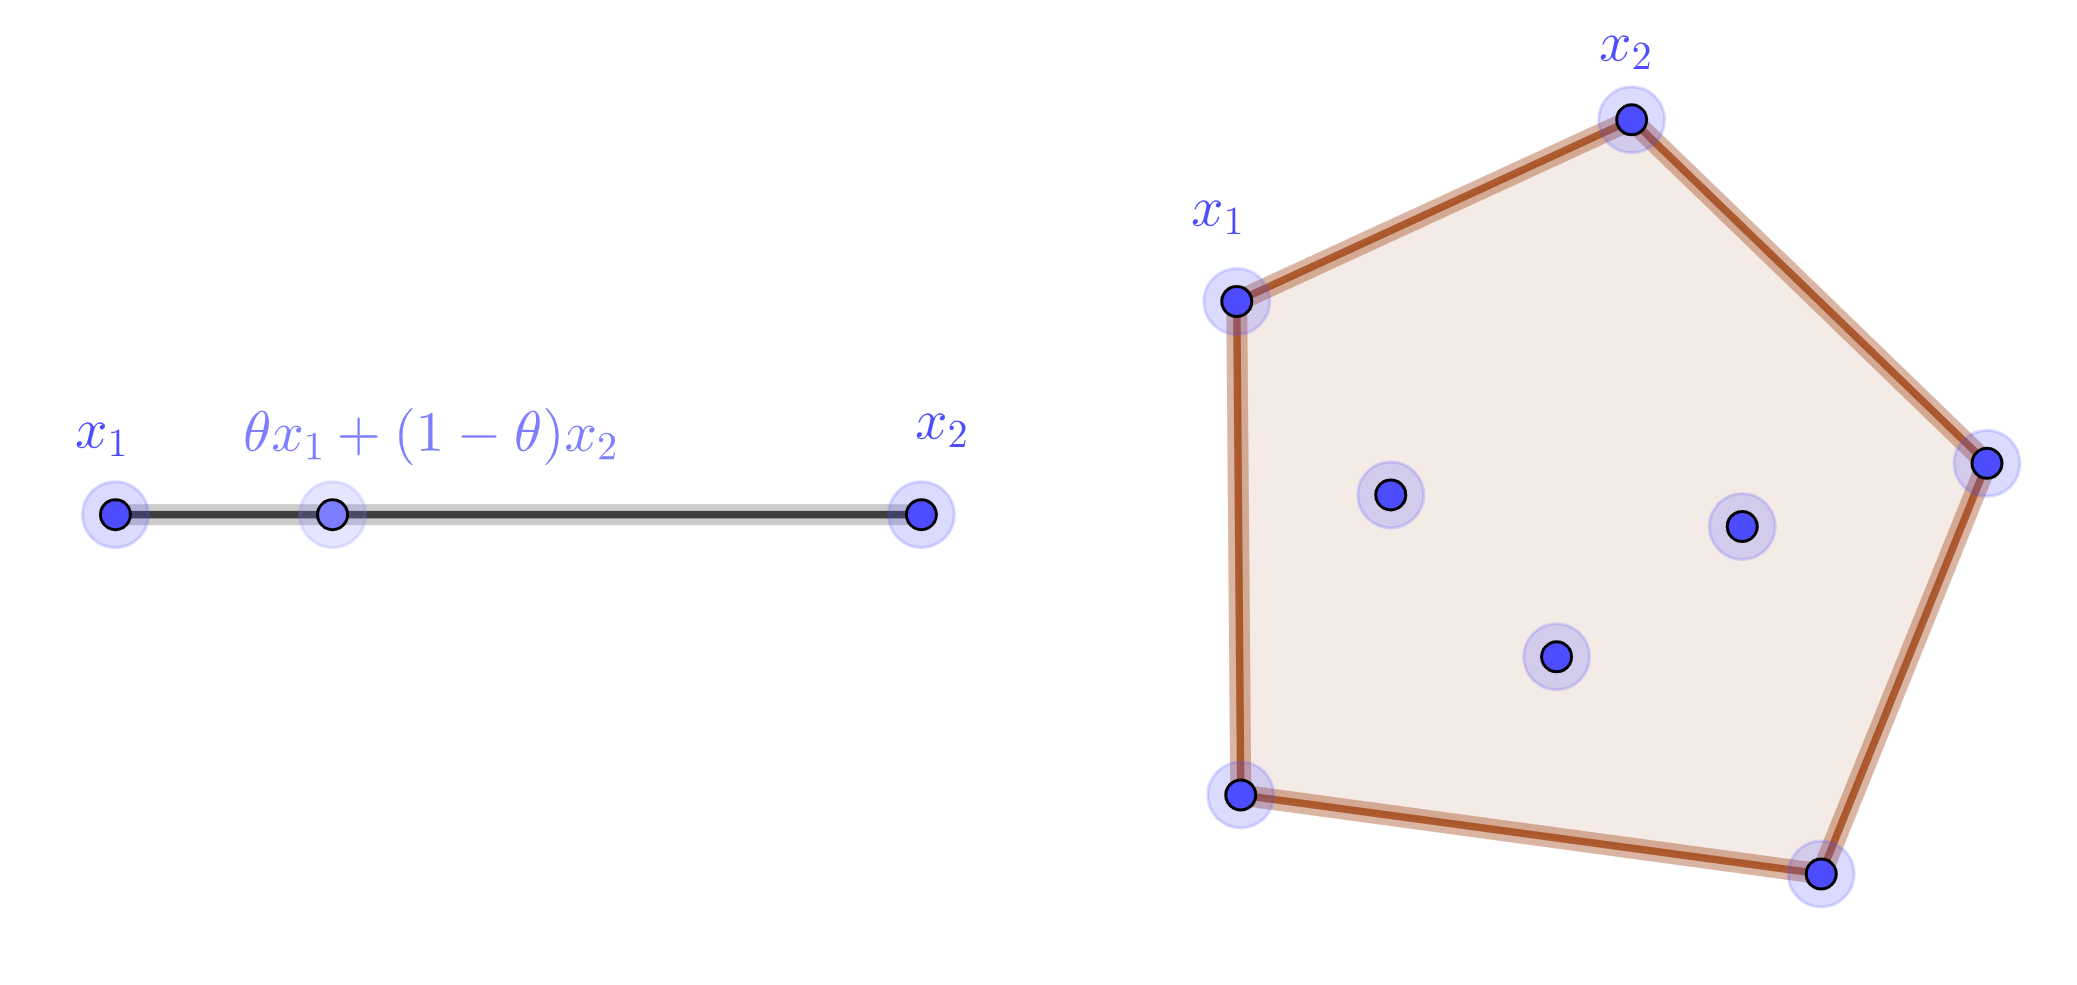
\includegraphics[width=9.5cm]{hinh_chuong2_convexfunc/chap2_line-convexhull.png}
	\caption{Hình mình họa đoạn thẳng (trái) và tập convex hull (phải) trong không gian 2D.}
	\label{fig:convexhull}	
\end{figure}

Các tập cơ bản như $\mathbf{R}^n$, $\mathbf{R}^n+ = \{x | x \in \mathbf{R}^n, x\geq 0\}$ là các tập lồi. 

Một số phép biển đổi bảo toàn tính lồi của tập hợp như sau:
\begin{itemize}
\item Giao của hai tập lồi là một tập lồi.
\item % should be in chap 1
Ảnh của một tập lồi $S$ cho bởi một hàm tuyến tính $f(x) = Ax+b$, $f(S)$ cũng là một tập lồi:
\begin{align*}
f(S) = \{f(x) | x\in S\}.
\end{align*}
\item % should be in chap 1
\textit{Nửa không gian} (half space) định nghĩa bởi $a^T x \leq b$, $x \in \mathbf{R}^n$ là một tập lồi.
\begin{figure}[h]
	\centering
	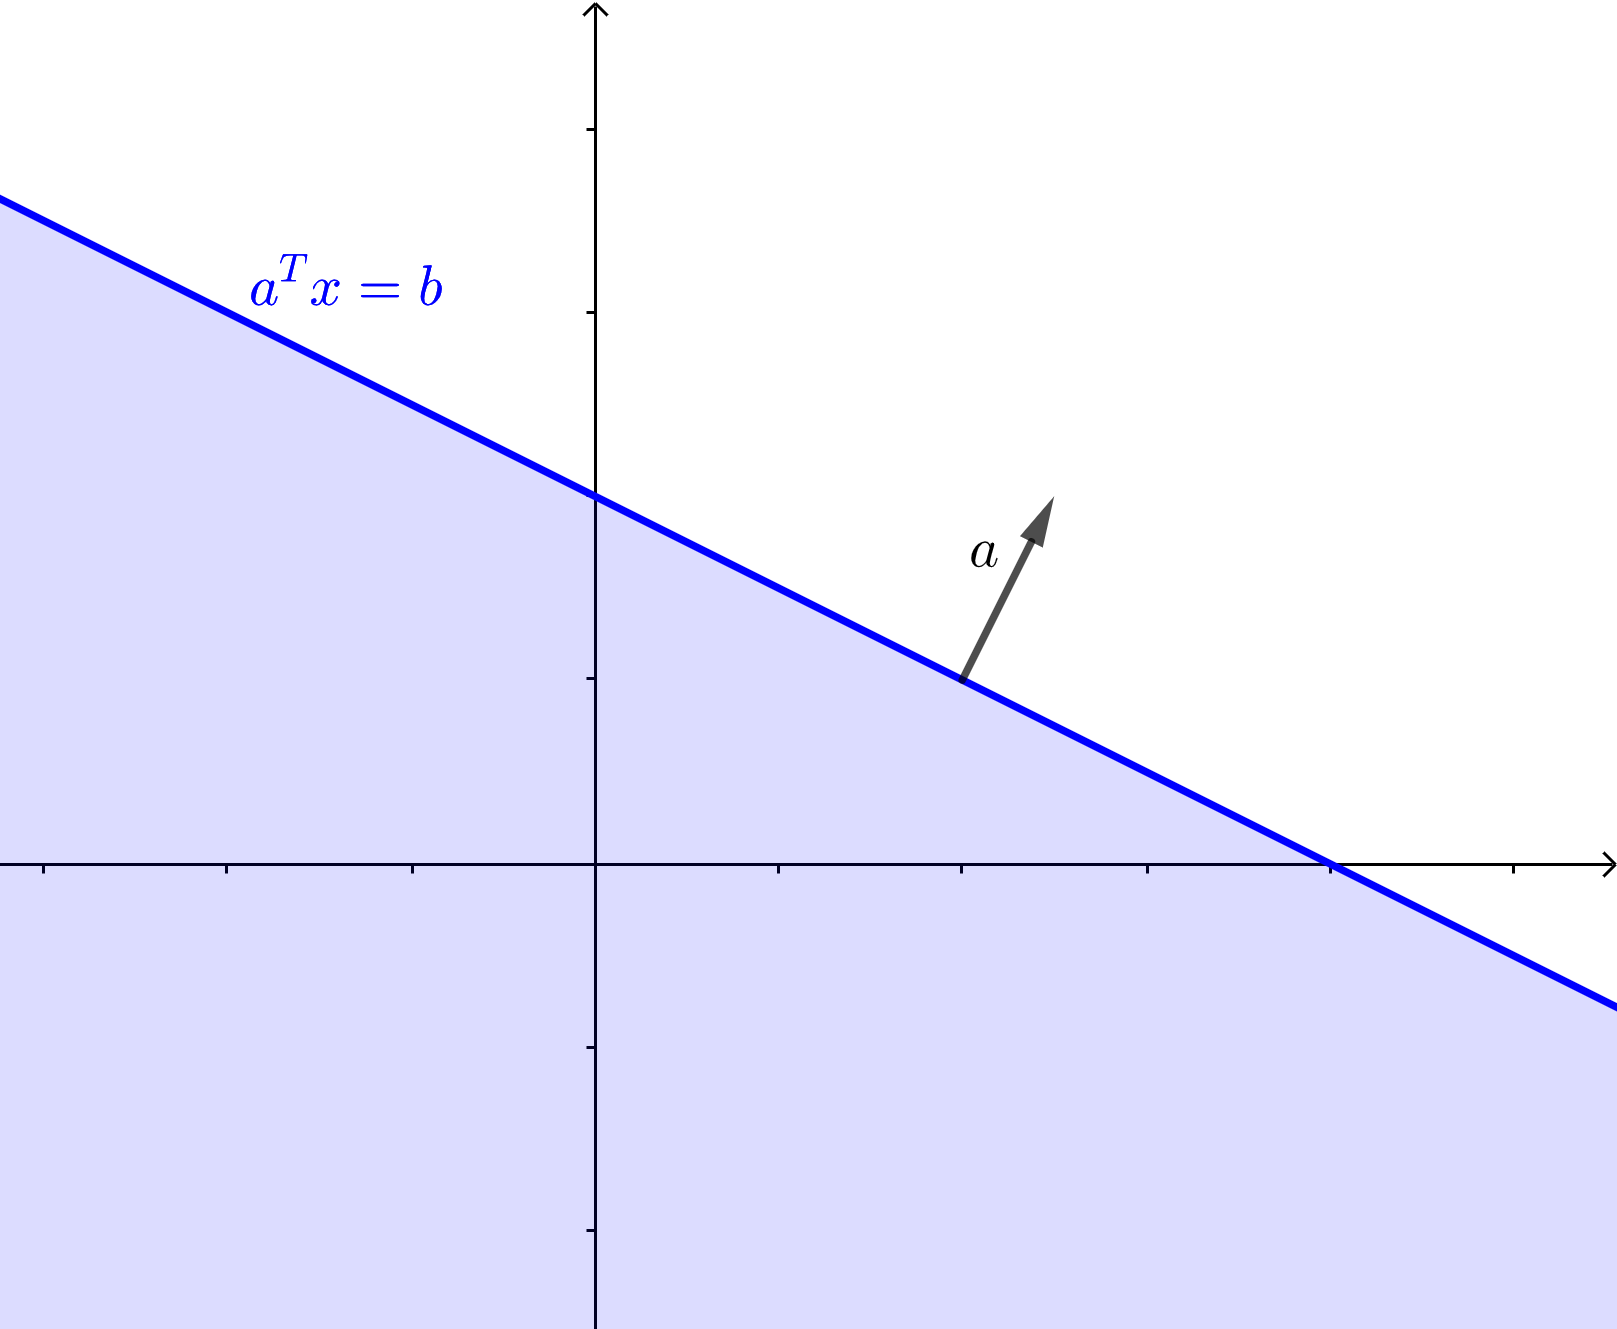
\includegraphics[width=7cm]{hinh_chuong2_convexfunc/chap2_halfspace.png}
	\caption{Nửa không gian tạo bởi $a^Tx \leq b$.}
	\label{fig:halfspace}	
\end{figure}
\item \textit{Đa điện} (polyhedron) được định nghĩa là tập hợp giao bởi các nửa không gian và siêu phẳng là tập lồi
\begin{align*}
\mathbf{P} = \{x | A x \leq b, C x  = d \}.
\end{align*}


\end{itemize}


\section{Hàm lồi}
\subsection{Định nghĩa}
Hàm số $f$ từ $\mathbf{R} \rightarrow \mathbf{R}$ là hàm lồi nếu miền xác định của $f$, $\rm{dom}f$ là một tập lồi và với hai vector bất kỳ $x, y \in \rm{dom}f$, ta có
\begin{align}
f(\theta x + (1-\theta) y) \leq \theta f(x) + (1- \theta) f(y), \forall \theta \in [0,1].
\label{eq:convex}
\end{align}

Hình \ref{fig:convexfunc} biểu diễn hàm lồi trong hệ trục $(x, f(x))$. Nếu hàm $f$ là hàm lồi thì các giá trị của $f$ trong đoạn $[x, y]$ luôn nhỏ hơn (nằm dưới) đoạn thẳng nối hai điểm $(x, f(x))$ và $(y, f(y))$.
\begin{figure}[h]
	\centering
	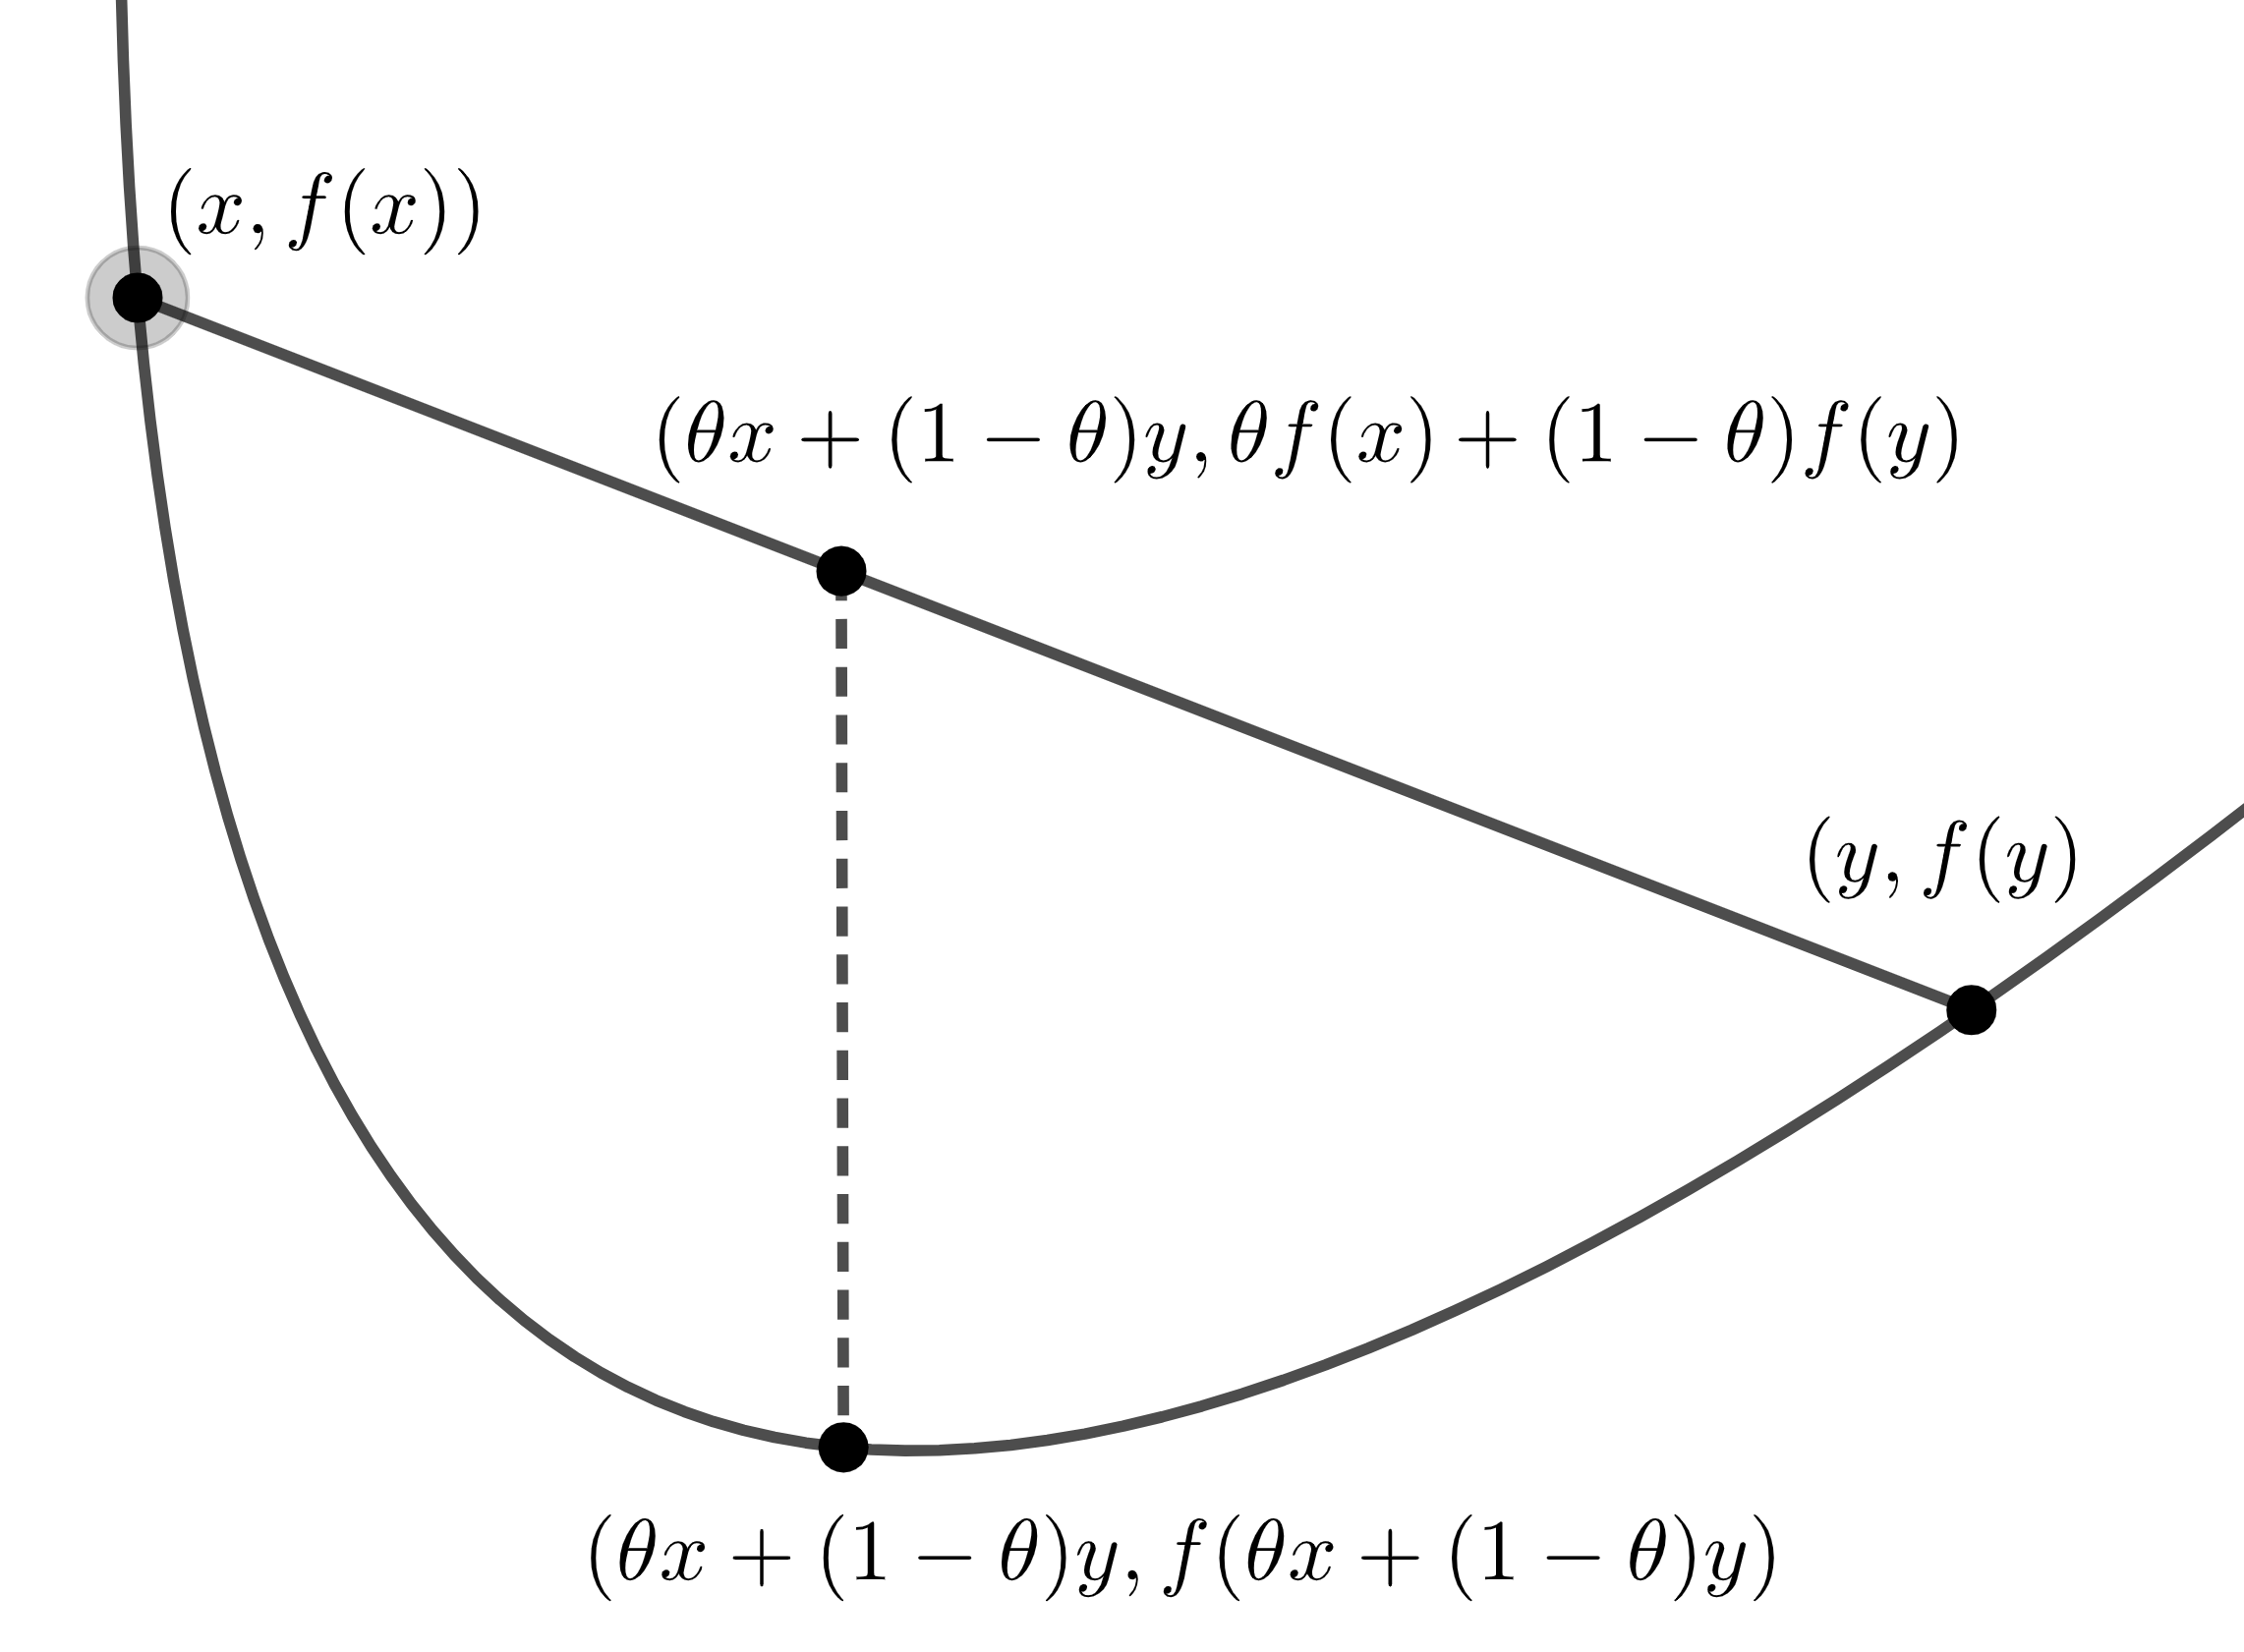
\includegraphics[width=8cm]{hinh_chuong2_convexfunc/chap2_convexfunc.png}
	\caption{Hình minh họa hàm lồi trong không gian 2D.}
	\label{fig:convexfunc}	
\end{figure}

Hàm $f$ được gọi là lồi chặt nếu bất đẳng thức \eqref{eq:chap2-convex} là dấu $<$ cho mọi $\theta \in (0,1)$.
Hàm lõm (concave) được định nghĩa ngược lại với hàm lồi. Một hàm số $f$ là lõm nếu $-f$ là một hàm lồi.

Một hàm số có thể vữa không lồi, vừa không lõm trên một tập xác định. Ví dụ hàm $f(x) = x^3$ không lồi và không lõm trên $\mathbf{R}$, tuy nhiên $f$ lồi trên tập số thực dương và lỏm trên tập số thực âm.

Ví dụ, ta có thể chứng minh hàm tuyến tính có dạng $f(x)=a^Tx+b$ là hàm lồi và cũng là hàm lõm theo định nghĩa. 
Mọi hàm norm đều là hàm lồi (bài tập). 

\noindent\fbox{\begin{minipage}{12cm}
\subsubsection*{Ghi chú: Norm}
\textit{Norms} (ký hiệu là $\|x\|$) thường được dùng như một ước lượng độ dài của một vector $x$. Khoảng cách giữa hai vector $x$ và $y$ được tính là $\|x-y\|$.

Hàm norm $f: \mathbb{R}^n \rightarrow \mathbb{R}$ được định nghĩa phải có những tính chất sau:
\begin{itemize}
\item $f(x) \geq 0, \forall x \in \mathbb{R}^n$
\item $f(x) = 0$ chỉ với $x = 0$ (tính xác định - definite)
\item $f(tx) = |t|f(x)$ với mọi $x \in \mathbb{R}^n$ and $t \in \mathbb{R}$ (tính đồng nhất - homogeneous)
\item $f(x+y) \leq f(x) + f(y)$.
\end{itemize}

Một số các hàm norm thông dụng như sau:
\begin{itemize}
\item $\ell_1$-norm (tổng trị tuyệt đối):
\begin{align*}
\|x\|_1 = |x_1| + |x_2| + \ldots + |x_n|.
\end{align*}
\item $\ell_\infty$-norm hay còn gọi Chebyshev:
\begin{align*}
\|x\|_\infty = \max\{|x_1|, |x_2|, \ldots , |x_n|\}.
\end{align*}
\item $\ell_2$-norm hay còn gọi Euclidean norm:
\begin{align*}
\|x\|_2 = (x^T x)^{1/2} = (x_1^2 + x_2^2 + \ldots + x_n^2)^{1/2}.
\end{align*}
\item $\ell_p$-norm, $p > 1$:
\begin{align*}
\|x\|_p = (x_1^p + x_2^p + \ldots + x_n^p)^{1/p}.
\end{align*}
\item Norm toàn phương (quadratic norm): cho ma trận $P$ xác định dương,
\begin{align*}
\|x\|_P = (x^T P x)^{1/2} = \|P^{1/2} x\|_2.
\end{align*}
%\item Norms in $\mathbb{R}^{m \times n}$: Frobenius norm, maximum-absolute-value norm.
\end{itemize}

\end{minipage}
}

\subsection{Điều kiện bậc một}

Giả sử hàm số $f$ khả vi\footnote{Hàm số khả vi tại điểm $x$ nếu nó tồn tại đạo hàm tại điểm đó.} tại mọi điểm trong miền xác định của nó $\rm{dom} f$. 
Hàm $f$ lồi nếu và chỉ nếu tập $\rm{dom} f$ lồi và 
\begin{equation}
f(y) \geq f(x) + \nabla f(x)^T (y-x), \forall x, y \in \rm{dom} f.
\label{eq:firstordercond_convex}
\end{equation}

Ý nghĩa đằng sau bất đẳng thức này được thể hiện trong Hình \ref{fig:firstordercond}. Hàm lồi luôn nằm trên tiếp tuyến của hàm số tại bất kỳ điểm $x$ nào.
\begin{figure}[h]
	\centering
	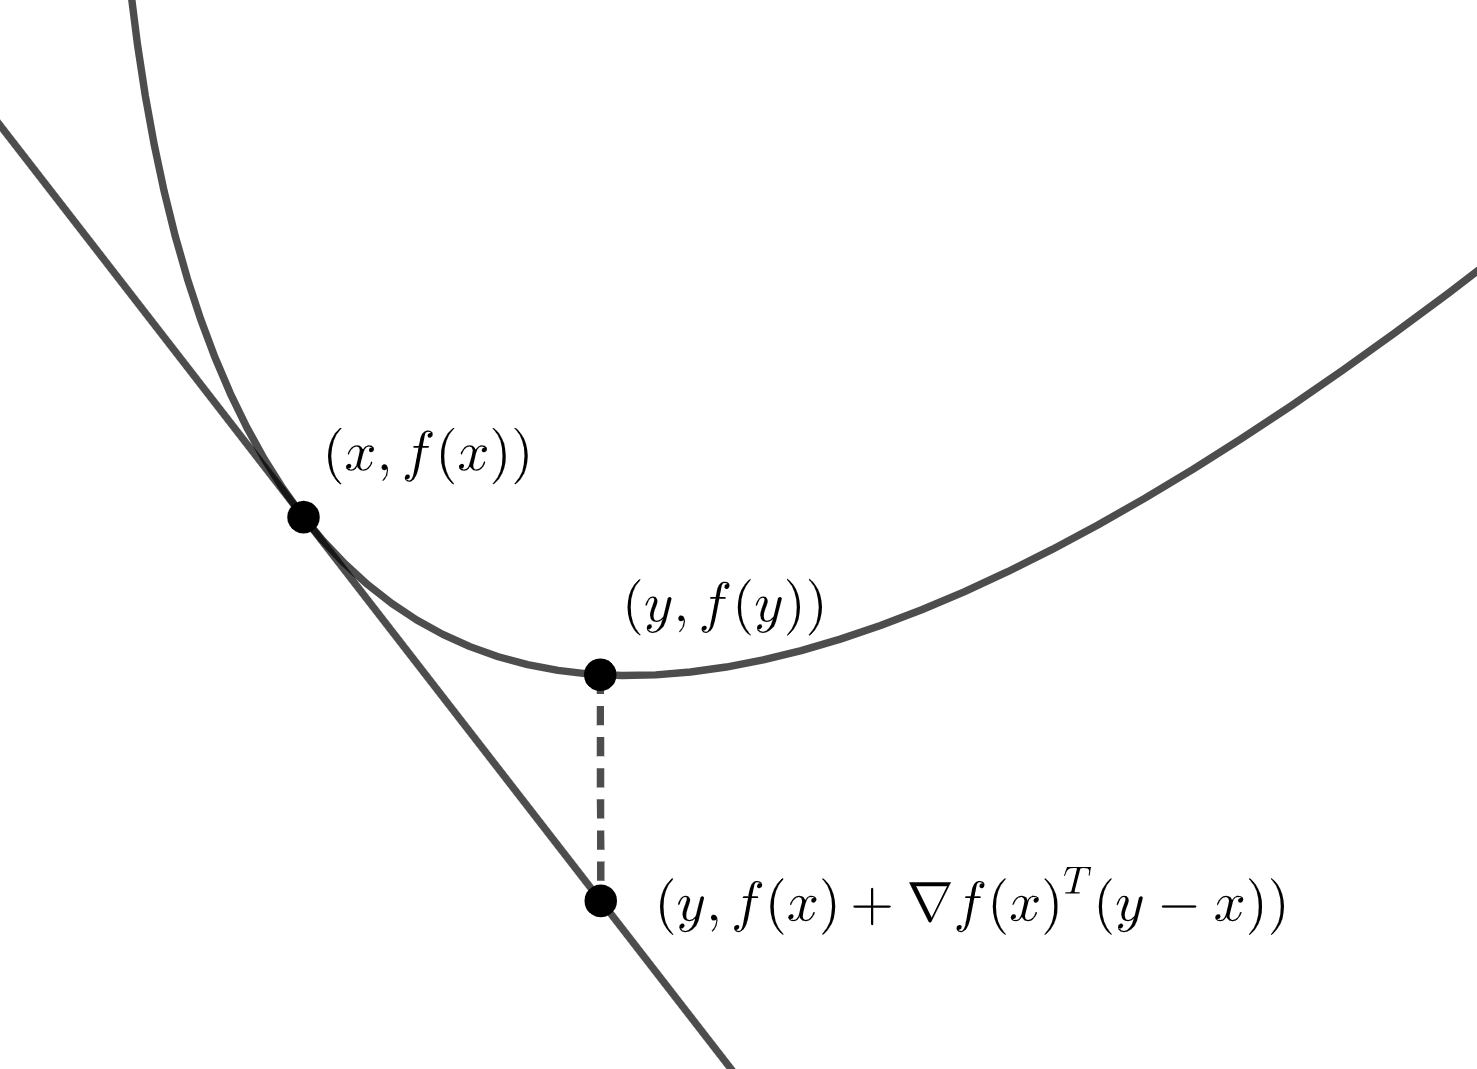
\includegraphics[width=8cm]{hinh_chuong2_convexfunc/chap2_firstordercond.png}
	\caption{Điều kiện bậc một để một hàm số là lồi khi $f(y) \geq f(x) + \nabla f(x)^T (y-x)$ cho mọi điểm $x, y$.}
	\label{fig:firstordercond}	
\end{figure}

Tương tự như vậy, điều kiện bậc một để một hàm số là lõm khi tập xác định $\rm{dom} f$ lồi và bất phương trình
\begin{equation}
f(y) \leq f(x) + \nabla f(x)^T (y-x)
\label{eq:firstordercond_concave}
\end{equation}
đúng cho mọi điểm $x, y \in \rm{dom} f$.

Hàm số được gọi là \textit{lồi chặt} (strictly convex) hay \textit{lõm chặt} (strictly concave) nếu các bất phương trình \eqref{eq:firstordercond_convex} và \eqref{eq:firstordercond_concave} không có dấu bằng.


\subsection{Điều kiện bậc hai}
Giả sử hàm $f$ có tồn tại đạo hàm bậc hai tại mọi điểm trong $\rm{dom} f$. 
Hàm $f$ lồi nếu và chỉ nếu ma trận Hessian là xác định dương.
\begin{equation}
\nabla^2 f(x) \geq 0, \forall x \in \rm{dom} f.
\end{equation}

\noindent\fbox{\begin{minipage}{12cm}
\subsubsection*{Ghi chú: Ma trận xác định dương}
Một ma trận $A \in \mathbf{R}^{n \times n}$ là xác định dương (positive semidefinite), ký hiệu là $A \geq 0$, nếu $x^T A x \geq 0$ với mọi vector $x \in \mathbf{R}^{n}$. Trong trường hợp $x^T A x >0$ với mọi $x$, ma trận $A$ được gọi là xác định dương chặt (positive definite).

Khái niệm về ma trận xác định âm (negative semidefinite) và xác định âm chặt (negative definite) là tương tự, chỉ có đổi dấu $\geq, >$ thành $\leq, <$.

Một số tính chất của ma trận bán xác định dương như sau:
\begin{itemize}
\item Một ma trận đối xứng là xác định dương nếu và chỉ nếu tất cả các \textit{giá trị riêng} (eigenvalue) của nó là số thực không âm. 
\item Một ma trận có thể vừa không xác định dương và cũng không xác định âm.
\item Nếu $A$ và $B$ là những ma trận xác đinh dương thì $A+B$ cũng xác định dương. Nếu $A$ hay $B$ xác định dương chặt thì $A+B$ xác định dương chặt.
\item Nếu $A$ xác định dương thì các phần tử trên đường chéo chính là số không âm.
%\item Nếu $A$ và $B$ là các ma trận đối xứng và xác định dương thì $C=[A_{ij}B_{ij}]$ cũng xác định dương.
\end{itemize}
\end{minipage}
}

Ta có thể chứng minh các hàm số sau là hàm lồi hoặc lõm bằng cách kiểm tra đạo hàm bậc hai:
\begin{itemize}
\item Hàm mũ $f(x) = e^{ax}, x \in \mathbf{R}$ lồi với mọi $a \in \mathbf{R}$ vì $f''(x) = a^2 e^{ax}$.

\item Hàm lũy thừa $f(x) = x^a$ lồi trên tập số thực dương khi $a\geq 1$ hoặc $a \leq 0$, và lõm khi $0 \leq a \leq 1$ vì $f''(x) = a(a-1)x^{a-2} \geq 0$ khi $a\geq 1$ hoặc $a \leq 0$ và ngược lại.

\item Hàm logarit $f(x) = \log(x)$ lõm trên tập số thực dương vì $f''(x) = -1/x^2 <0$.

\item Hàm entropy $f(x) = -x\log (x)$ là hàm lõm trên tập số thực dương.

\item Hàm log-sum-exp $LSE(x_1,...,x_n) = \log(\sum_{i=1}^n e^{x_i})$ là hàm lồi. 
\begin{align*}
\nabla^2 f(x) = \frac{1}{1^Tz} diag(z) - \frac{1}{(1^z)^2}zz^T \succeq 0
\end{align*}
trong đó $z_k = exp(x_k)$. (Vui lòng xem chứng minh ma trận $v^T\nabla^2 f(x)v$ xác định dương với mọi $v$ trong sách \cite{boyd}.)
\end{itemize}

\subsubsection*{Hàm toàn phương}
Hàm $f(x_1, x_2) = 10 x_1^2 + x_2^2$, trong đó $x_1, x_2 \in \mathbf{R}$ là hàm lồi 
bởi vì $\nabla^2 f = \begin{bmatrix}&10 & 0 \\&0 &1 \end{bmatrix}$ là ma trận xác định dương.

Hàm toàn phương tổng quát có dạng
\begin{equation}
f(x) = (1/2) x^T P x + q^T x + r,
\end{equation}
trong đó $x, q$ là các vector $n$ chiều, $P$ là ma trận đối xứng bậc $n$, và $r$ là số thực.

Ta có, $\nabla f(x) = Px + q$ và $\nabla^2 f(x) = P$.
Do đó, hàm toàn phương $f(x)$ lồi nếu và chỉ nếu $P$ là ma trận xác định dương.


\section{Một số tính chất của hàm lồi}

\subsection*{Tổng các hàm lồi}
Cho $w_1,...,w_m$ là các số thực không âm. Nếu $f_1(x),...,f_n(x)$ là các hàm lồi thì 
\begin{align*}
f(x) &= w_1 f_1(x) + \ldots + w_m f_m(x).
\end{align*}
lồi.
Mở rộng ra, ta có
\begin{align*}
g(x) &= \int_A w(y)f(x, y) dy,
\end{align*}
là hàm lồi nếu $f(x)$ lồi và $w(y) \geq 0, \forall y \in A$.

\subsection*{Biến đổi tuyến tính}
Giả sử $g(x) = f(Ax + b)$, trong đó $A \in \mathbb{R}^{n \times m}, b \in \mathbb{R}^n$. 
%Define $g: \mathbb{R}^m \rightarrow \mathbb{R}$, .
Nếu $f$ là hàm lồi (hoặc lõm), thì $g$ cũng là hàm lồi (hoặc lõm).

Ví dụ hàm log barrier dùng cho các ràng buộc là bất phương trình tuyến tính là hàm lồi trên tập mà $f(x)$ xác định
\begin{align*}
f(x) = - \sum^m_{i=1} \log(b_i - a^T_i x).
\end{align*}
Hay hàm norm dùng trong bài toán hồi quy tuyến tính (linear regression)
\begin{align*}
f(x) = \| Ax - b\|
\end{align*}
là hàm lồi, trong đó $A \in \mathbb{R}^{m \times n}, b \in \mathbb{R}^m$.

\subsection*{Hàm cực đại, cực tiểu}
Giả sử hai hàm số $f_1, f_2$ là các hàm lồi. Hàm được định nghĩa cực đại $f(x) = \max\{f_1(x), f_2(x)\}$, trên miền xác định $\mathbf{dom}f = \mathbf{dom}f_1 \cap \mathbf{dom}f_2 $ cũng là hàm lồi.

Áp dụng tính chất trên, ta có các hàm sau đều là hàm lồi:
\begin{itemize}
\item $f(x) = \max_i \|A^{(i)} x - b^{(i)}\|$, trong đó $A^{(i)} \in \mathbb{R}^{m \times n}, b^{(i)} \in \mathbb{R}^m$, và $\|.\|$ là norm.
\item $f(x) = \max\{a_1^T x + b_1, \ldots, a_n^T x + b_n\}$ 
\item $f(x) = \max\{x_1, \ldots, x_n\}$ $x_1, \ldots, x_n \in \mathbb{R}^n$.
\end{itemize}

Nếu $f(x,y)$ lồi, và $C$ là tập lồi thì $g(x) =\min_{y \in C} f(x, y)$ là hàm lồi.

\subsection*{Luật kết hợp}
Cho các hàm số $g: \mathbf{R}^n \rightarrow \mathbf{R}, h: \mathbf{R} \rightarrow \mathbf{R}$, hàm số được định nghĩa bởi
\begin{align*}
f(x) = h(g(x))
\end{align*}
\begin{itemize}
\item lồi nếu $h$ lồi và không giảm, $g$ lồi,
\item lồi nếu $h$ lồi và không giảm, $g$ lõm,
\item lõm nếu $h$ lõm và không giảm, $g$ lõm,
\item lõm nếu $h$ lõm và không tăng, $g$ lồi.
\end{itemize}

Ta nhớ các quy tắc trên bằng cách xem xét trường hợp đặc biệt khi $n=1$:
\begin{align*}
f''(x) = h''(g(x))g'(x)^2 + h'(g(x))g''(x).
\end{align*}
$f'' \geq 0$ ($f$ lồi) nếu 
\begin{itemize}
\item $h'' \geq 0$ ($h$ lồi) và $h' \geq 0$ ($h$ không giảm) và $g''(x) \geq 0$ ($g$ lồi), hoặc 
\item $h'' \geq 0$ ($h$ lồi) và $h' \ leq 0$ ($h$ không tăng) và $g''(x) \leq 0$ ($g$ lõm).
\end{itemize}
$f'' \leq 0$ ($f$ lõm) nếu 
\begin{itemize}
\item $h'' \leq 0$ ($h$ lõm) và $h' \geq 0$ ($h$ không giảm) và $g''(x) \leq 0$ ($g$ lõm), hoặc 
\item $h'' \leq 0$ ($h$ lõm) và $h' \ geq 0$ ($h$ không giảm) và $g''(x) \geq 0$ ($g$ lồi).
\end{itemize}

Từ các quy tắc kết hợp trên, ta có thể suy ra ngay rằng:
\begin{itemize}
\item Nếu $g$ lồi thì $e^{g(x)}$ lồi.
\item Nếu $g$ lõm và dương, thì $\log g(x)$ lõm.
\item Nếu $g$ lõm và dương, thì $1/g(x)$ lồi.
\item Nếu $g$ lồi, không âm, và $p \geq 1$, thì $g(x)^p$ lồi.
\item Nếu $g$ lồi, thì $-\log(-g(x))$ lồi trên tập $\{x | g(x) <0\}$.
\item $\log(\sum_{i=1}^n e^{y_i})$ là hàm lồi, do đó, $f(x) = -\log(-\log(\sum_{i=1}^m e^{a_i^T x + b_i}))$ là hàm lồi trên tập $\{x | \sum_{i=1}^m e^{a_i^T x + b_i} < 1 \}$. 
\end{itemize}

\subsection*{Tập $\alpha$-sublevel}
\emph{Level set} của một hàm $f(x)$ là tập hợp các đường cong mà $f(x)$ là một hằng số.
Ta thấy level set được biểu diễn trong các bản đồ để thể hiện độ cao núi hay độ sâu của biển, hồ.

\emph{Tập hợp $\alpha$-sublevel} của một hàm $f$ được định nghĩa bởi
\begin{align*}
\{x | x \in \mathrm{dom} f, f(x) \leq \alpha \}.
\end{align*}
Sublevel set của một hàm lồi là tập lồi, tuy nhiên ngược lại thì không đúng. 
Nếu một hàm mà tất các các sublevel set là lồi thì ta chỉ kết luận được hàm đó là hàm quasiconvex. 
(Vui lòng tham khảo thêm về hàm quasiconvex trong \cite{boyd}.)

\begin{figure}[h]
	\centering
	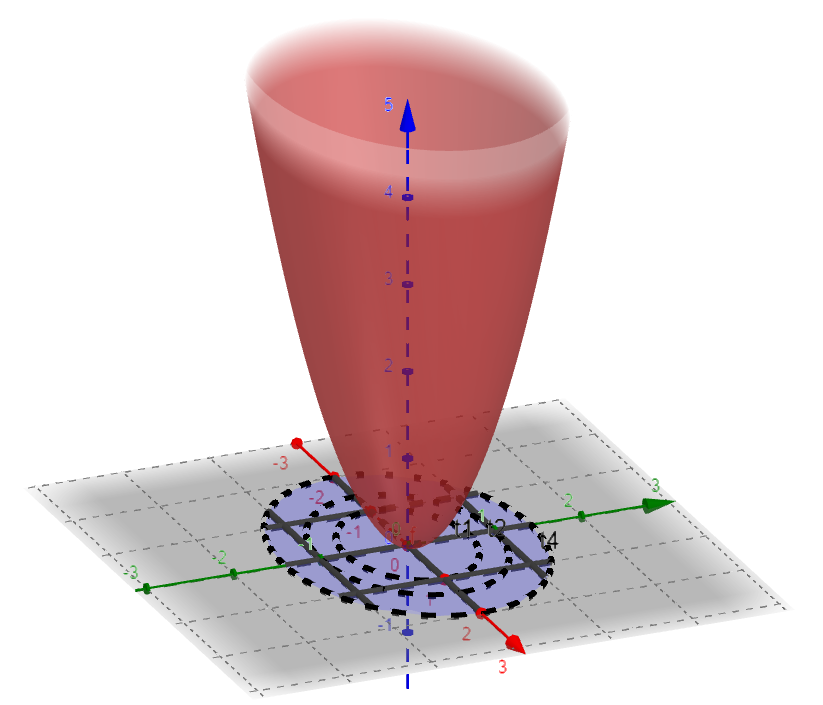
\includegraphics[width=5.5cm]{hinh_chuong2_convexfunc/chap2_levelset_3d.png}	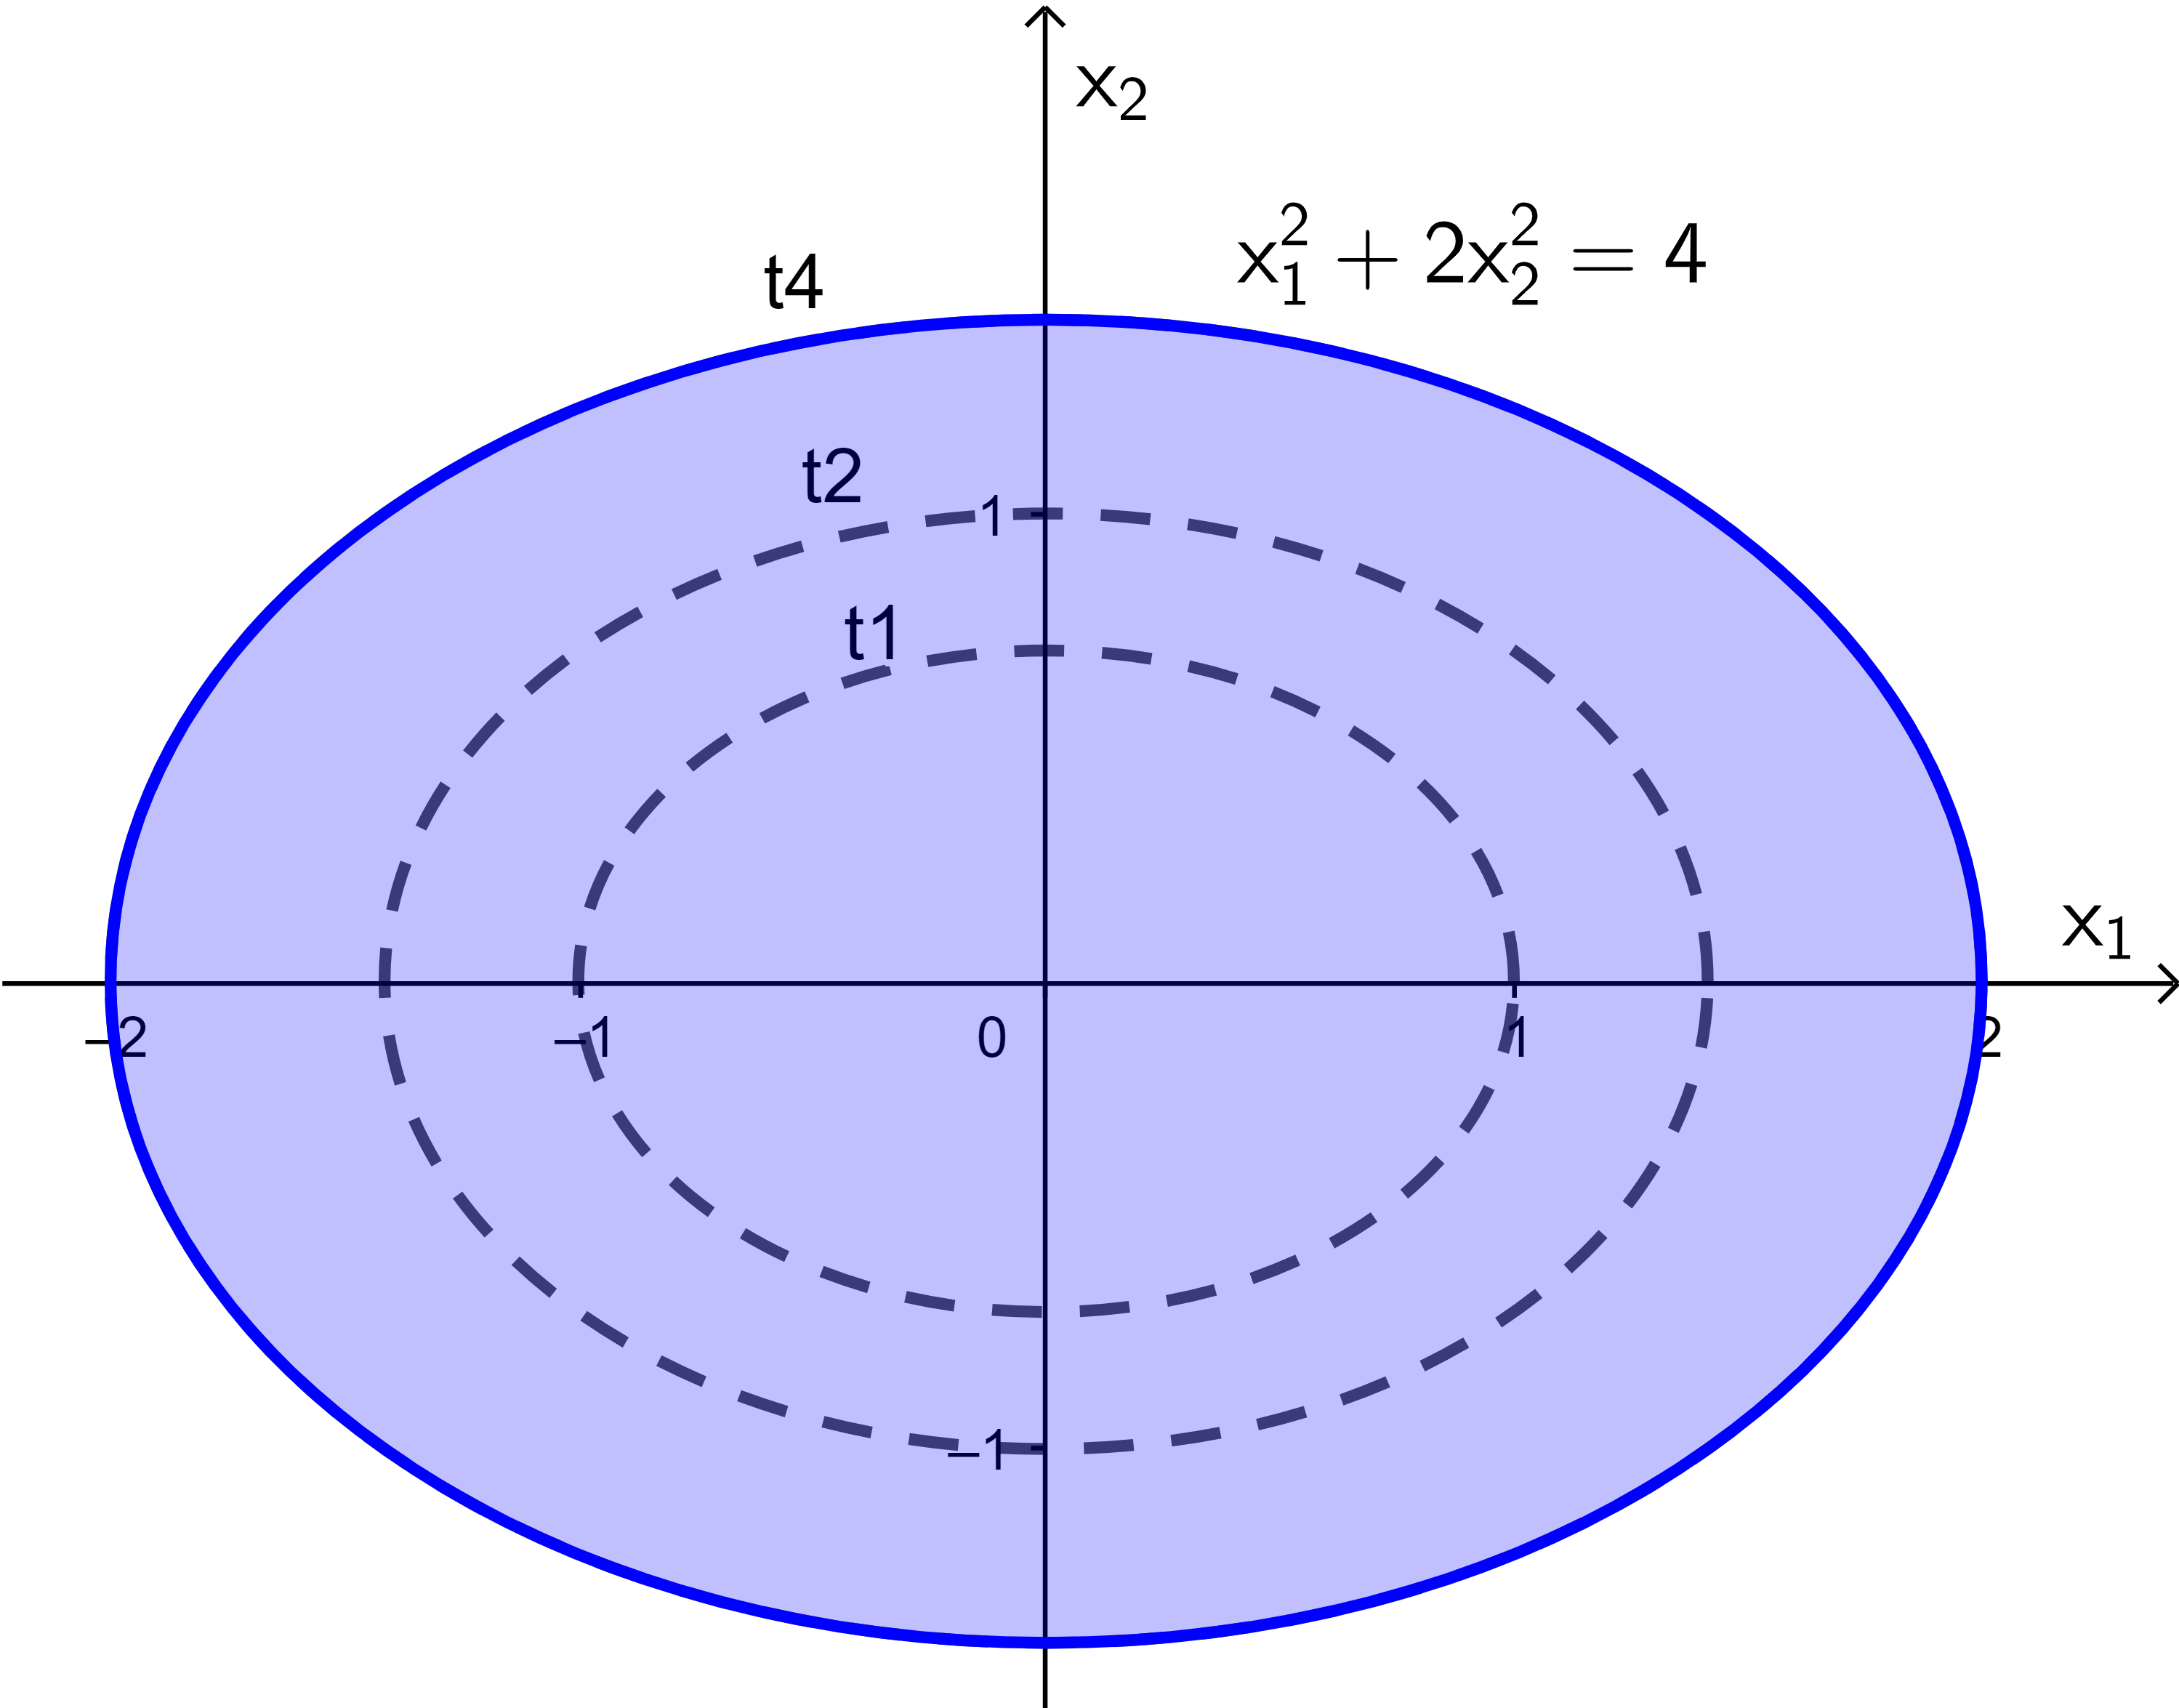
\includegraphics[width=5cm]{hinh_chuong2_convexfunc/chap2_levelset_2d.png}

	\caption{Hình biểu diễn hàm $f(x_1,x_2) = 4x_1^2 + 5x_2^2$ trong không gian 3D (hình bên trái) và các level set t1, t2, và t4 của hàm $f$ với các giá trị $f(x_1,x_2) = $1, 2 và 4 tương ứng (hình bên phải). Miền được tô đậm là 4-sublevel set của hàm số $f$.}
	\label{fig:epigraph}	
\end{figure}

\subsection*{Epigraph}
Cho hàm $f(x): \mathbf{R}^n \rightarrow \mathbf{R}$. Epigraph của hàm $f$ là tập hợp
\begin{align*}
\mathrm{epi} f = \{(x,t) | x \in \mathrm{dom} f, f(x) \leq t \}.
\end{align*}
Ta có, \emph{$f$ là một hàm lồi nếu và chỉ nếu epigraph là một tập lồi với mọi $t \in \mathbf{R}$} (Hình \ref{fig:epigraph}).

\begin{figure}[h]
	\centering
	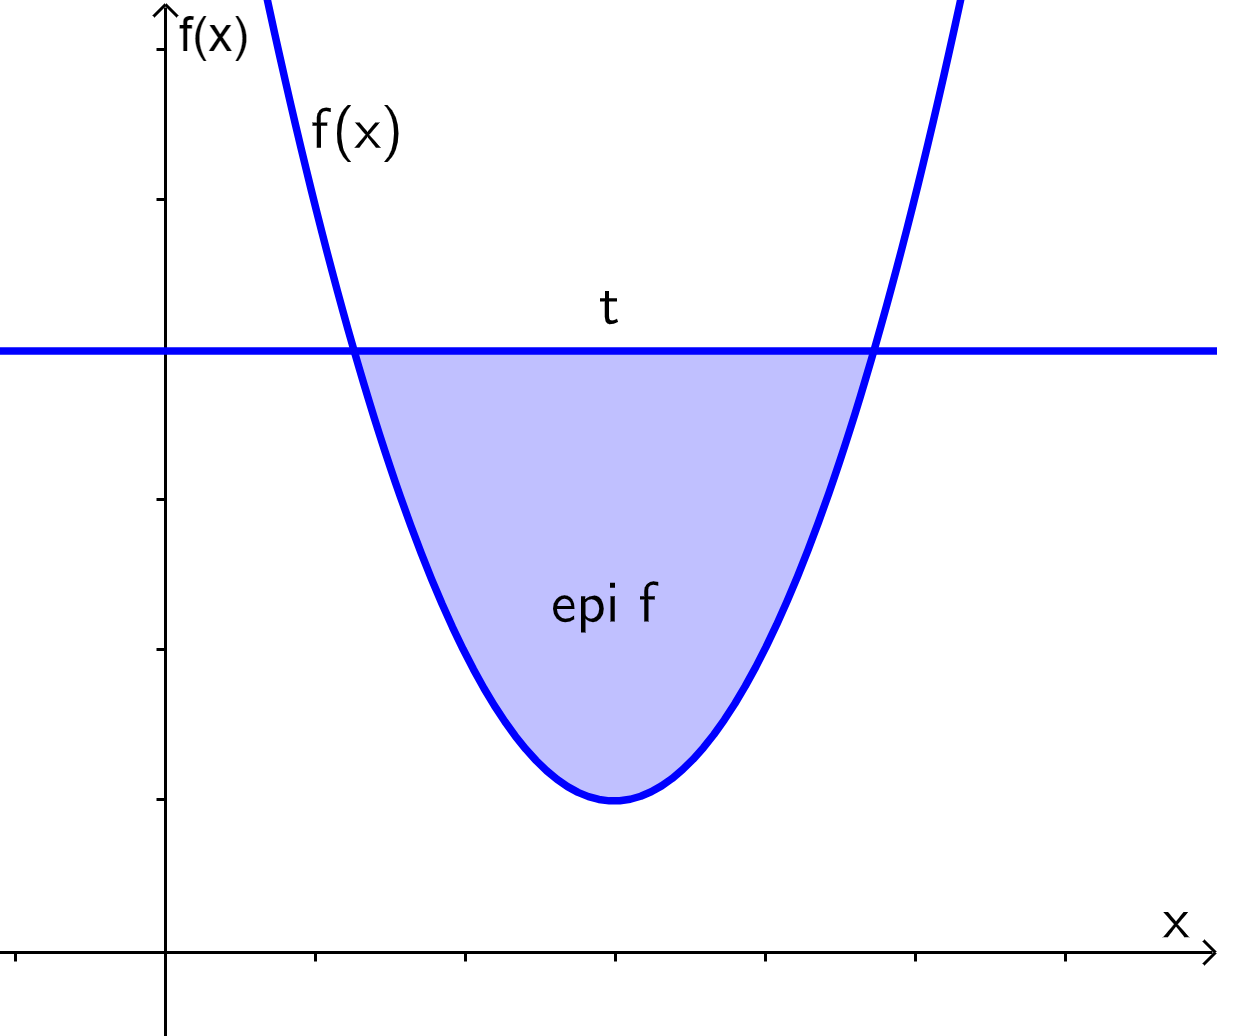
\includegraphics[width=5cm]{hinh_chuong2_convexfunc/chap2_epigraph.png}
	\caption{Epigraph của hàm $f$.}
	\label{fig:epigraph}	
\end{figure}

%\subsubsection*{Perspective}
%Phối cảnh (perspective) của $f:  \mathbb{R}^{n} \rightarrow \mathbb{R}$ là hàm $g: \mathbb{R}^{n+1} \rightarrow \mathbb{R}$ định nghĩa bởi
%\begin{align*}
%g(x, t) = t f(x/t), \forall t >0.
%\end{align*}
%Nếu $f$ lồi (hay lõm) thì hàm phối cảnh $g$ cũng là hàm lồi (hoặc lõm).
%
%Áp dụng tính chất trên ta có:
%\begin{itemize}
%\item Do $f(x) = x^T x$ lồi, nên $g(x, t) = x^T x/t$ lồi trên miền $t >0$
%\item Do $f(x) = -\log(x)$ lồi, nên entropy $g(x,t) = t\log(t) - t\log(x)$ cũng lồi.
%\item Nếu $f$ là hàm lồi , thì
%\begin{align*}
%g(x) = (c^Tx + d) f((Ax+b)/(c^Tx + d))
%\end{align*} 
%lồi trên tập $\{ x| c^Tx + d >0, (Ax+b)/(c^Tx + d) \in dom(f) \}$
%\end{itemize}

\section{Hàm quasiconvex}
Hàm số $f$ là \emph{quasiconvex} (quasi có nghĩa là gần như, tựa như, nên loại hàm này có thể dịch là \emph{hàm tựa lồi}) nếu tập xác định và tất cả các sublevel set của nó đều là tập lồi.

Hàm $f$ được gọi là \emph{quasiconcave} nếu $-f$ là quasiconvex.
Một hàm vừa quasiconvex, vừa quasiconcave thì được gọi là \emph{quasilinear}.
Tất cả các hàm lồi đều là quasive convex. Tuy nhiên điều ngược lại thì không đúng.

Ví dụ các hàm sau là hàm quasi-:
\begin{itemize}
\item $\mathrm{ceil}(x) = \min\{ z \in \mathbf{Z} | z \geq z \}$ là quasiconvex.
\item $f: \mathrm{R}^2 \rightarrow \mathbf{R}$, $f(x_1, x_2) = x_1 x_2$ là quasiconcave trên tập số không âm $\mathrm{R}^2$ vì tập superlevel set $x_1 x_2 >= \alpha$ lồi trên tập $\mathbf{R}^2$.
\item $f(x) = \frac{||x-a||_2}{||x-b||_2}$ là quasiconvex trên tập $\{x | ||x-a||_2 \leq ||x-b||_2\}$.
\end{itemize}

\begin{figure}[h]
	\centering
	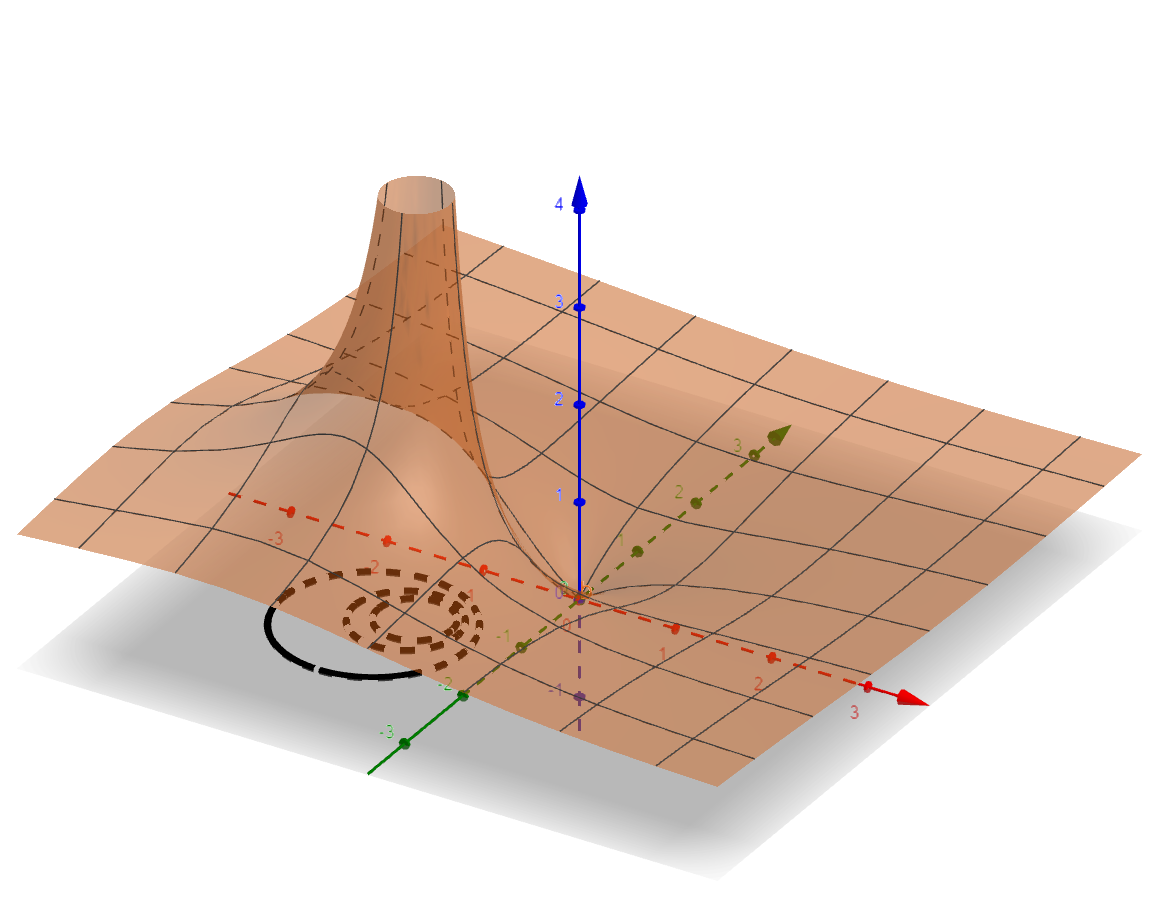
\includegraphics[width=6cm]{hinh_chuong2_convexfunc/chap2_quasiconvex_3d.png}
	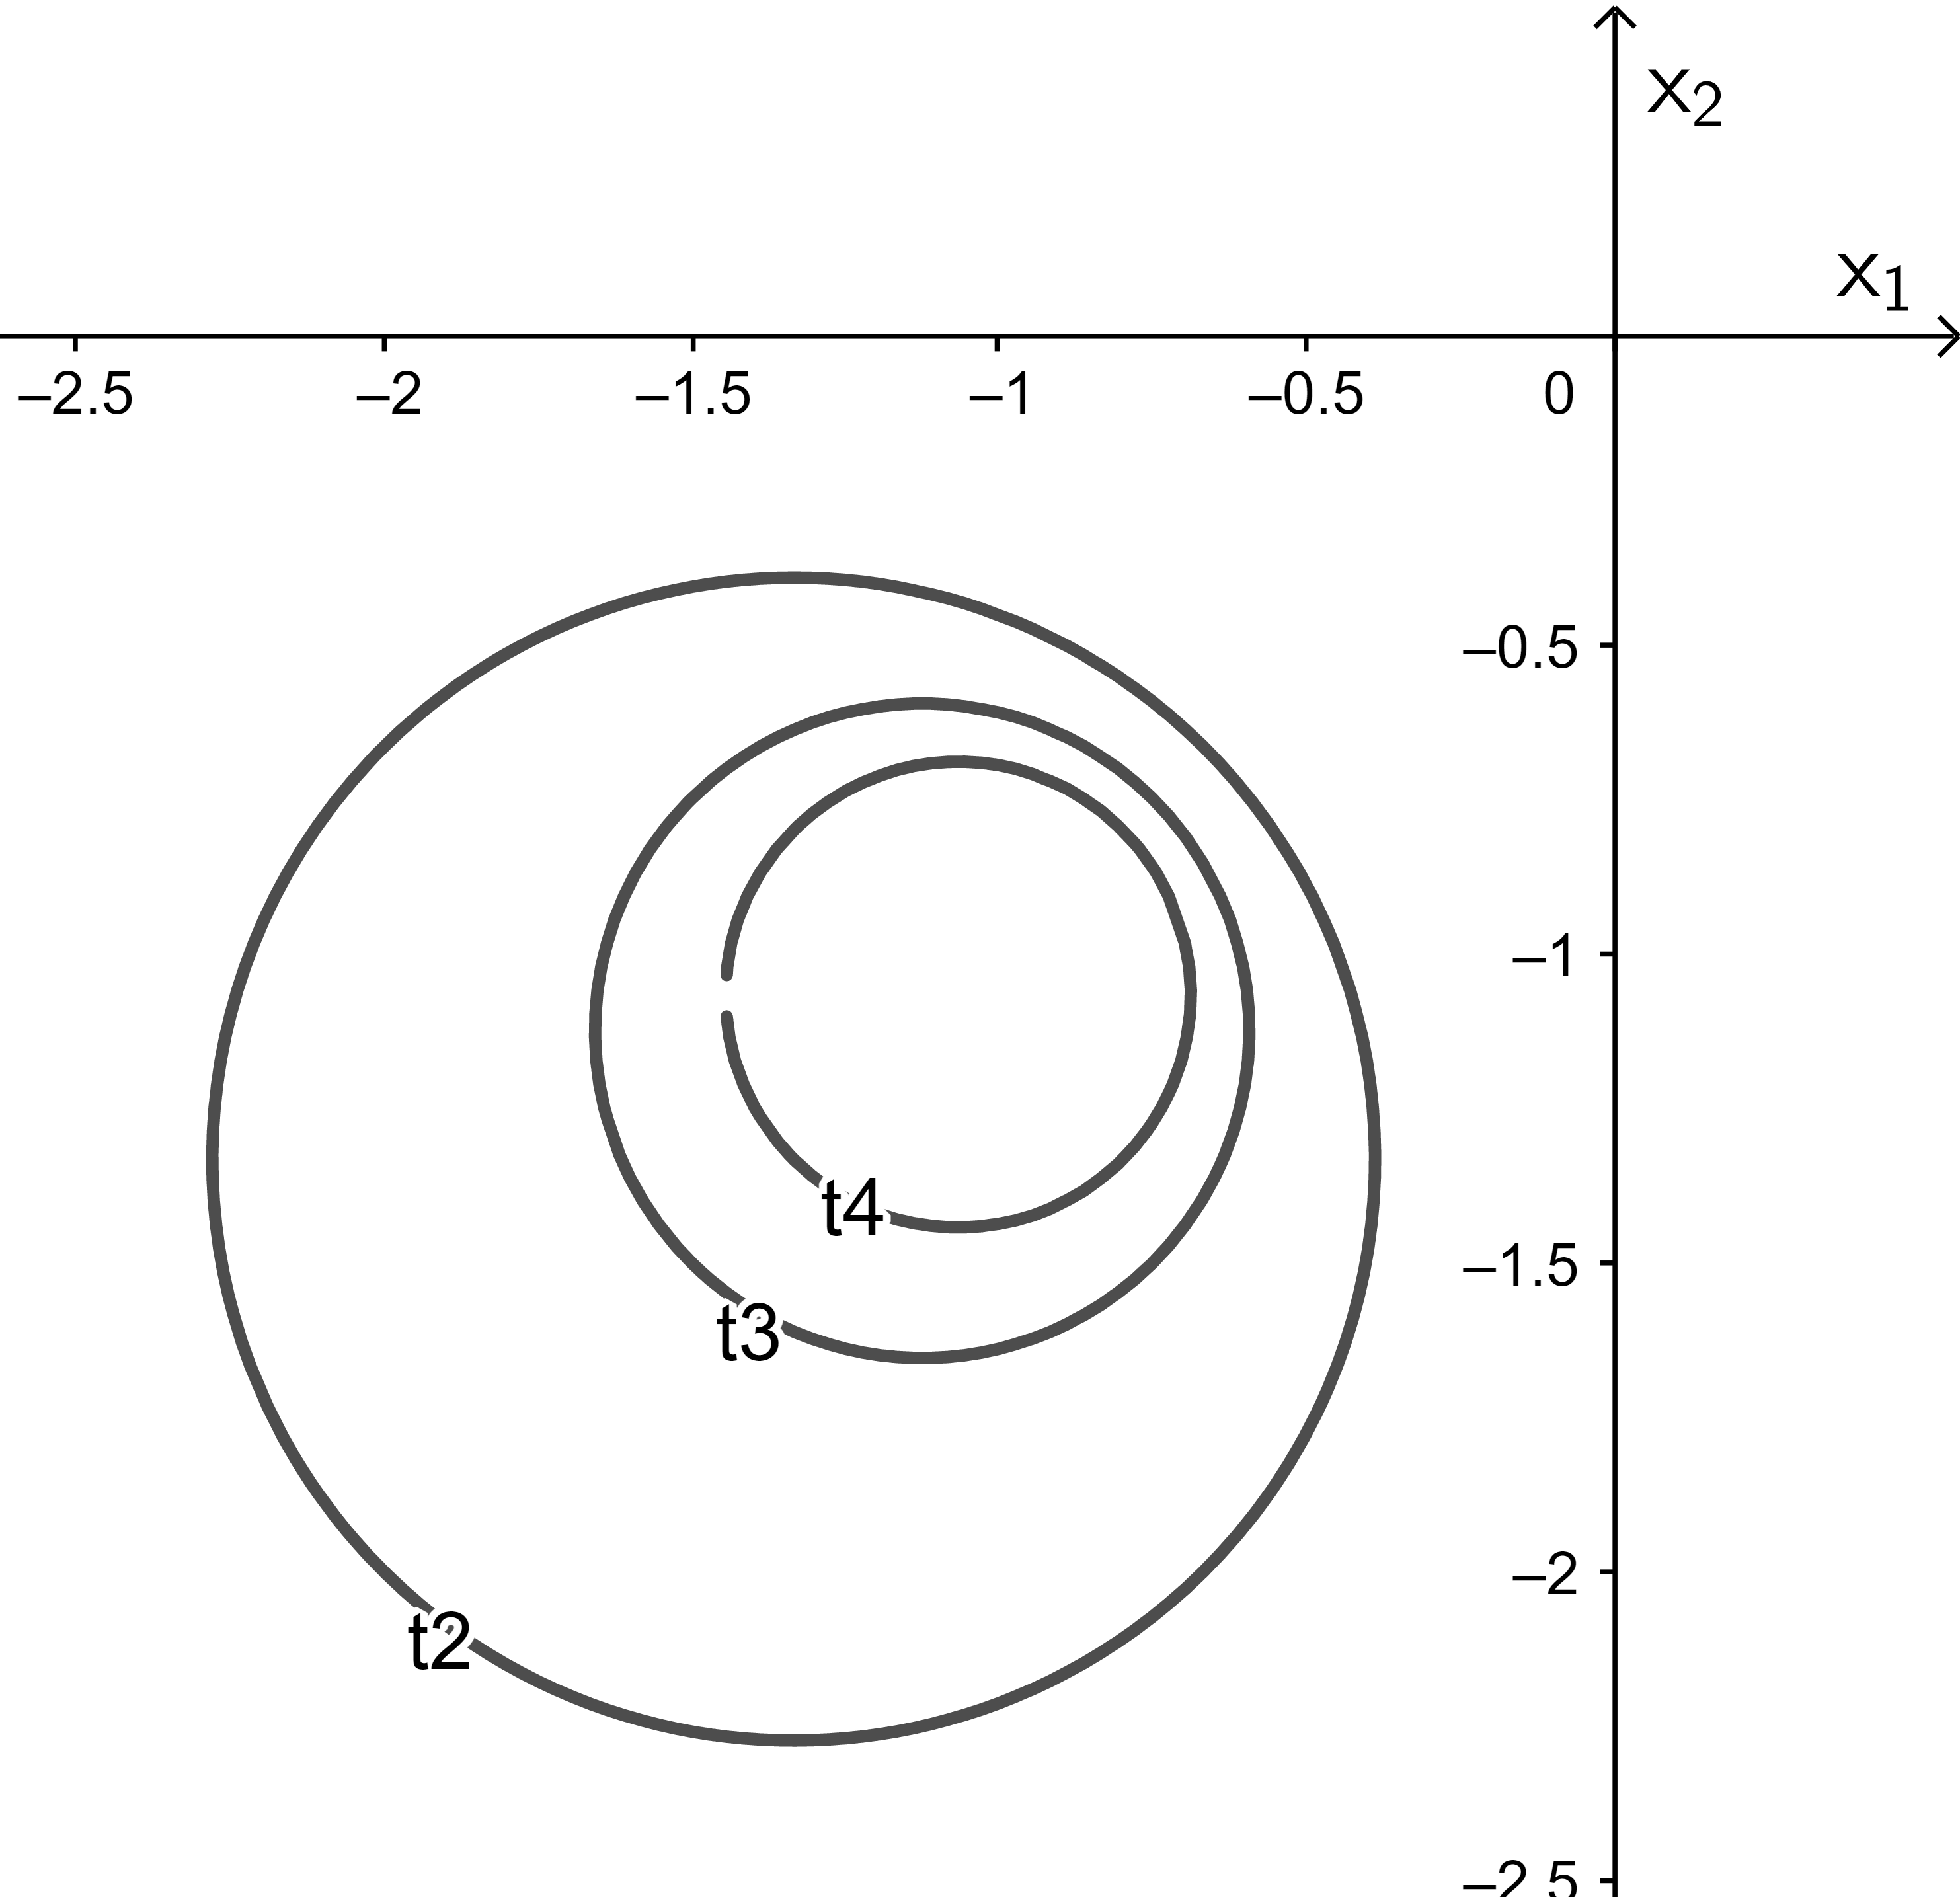
\includegraphics[width=5cm]{hinh_chuong2_convexfunc/chap2_quasiconvex_2d.png}
	\caption{Biểu diễn hàm $f(x_1,x_2) = \frac{||x-a||_2}{||x-b||_2}$, trong đó $a=(0,0), b=(-1,-1)$ trong không gian 3D (hình bên trái) và sublevel set t2, t3, và t4 trong không gian 2D tương ứng với $f(x_1,x_2) = 2$, 3, và 4 (hình bên phải).}
	\label{fig:quasiconvex}	
\end{figure}

Hàm quasiconvex xuất hiện trong một số ứng dụng trong thực tế kinh tế, viễn thông,... Mặc dù không thông dụng như tối ưu lồi, tối ưu hàm quasiconvex cũng là một nhánh của lý thuyết tối ưu, tuy nhiên nó không được đề cập đến trong khuôn khổ sách này.

\section{Hàm log-concave và log-convex}
Hàm $f$ dương là log-concave nếu $\log f$ là hàm lõm
\begin{align*}
f(\theta x + (1-\theta)y) \geq f(x)^\theta f(y)^{1-\theta}, \forall 0 \leq \theta \leq 1.
\end{align*}
Tương tự như vậy, $f$ là log-convex nếu $\log f$ lồi.

Ví dụ, hàm mũ $x^a$ xác định trên tập số thực dương là log-convex với mọi $a \leq 0$ và log-concave với mọi $a \geq 0$.

\subsection*{Hàm sigmoid} 
Hàm \textit{sigmoid} $\mathbf{R}^n \rightarrow \mathbf{R}$, hay còn được gọi là hàm logistic, được dùng để biểu diễn xác suất trong bài toán phân hai lớp là log-concave (Hình \ref{fig:sigmoid})
\begin{align*}
sigmoid(x) = \frac{1}{1 + e^{-w^T x}}
\end{align*}
\begin{figure}[h]
	\centering
	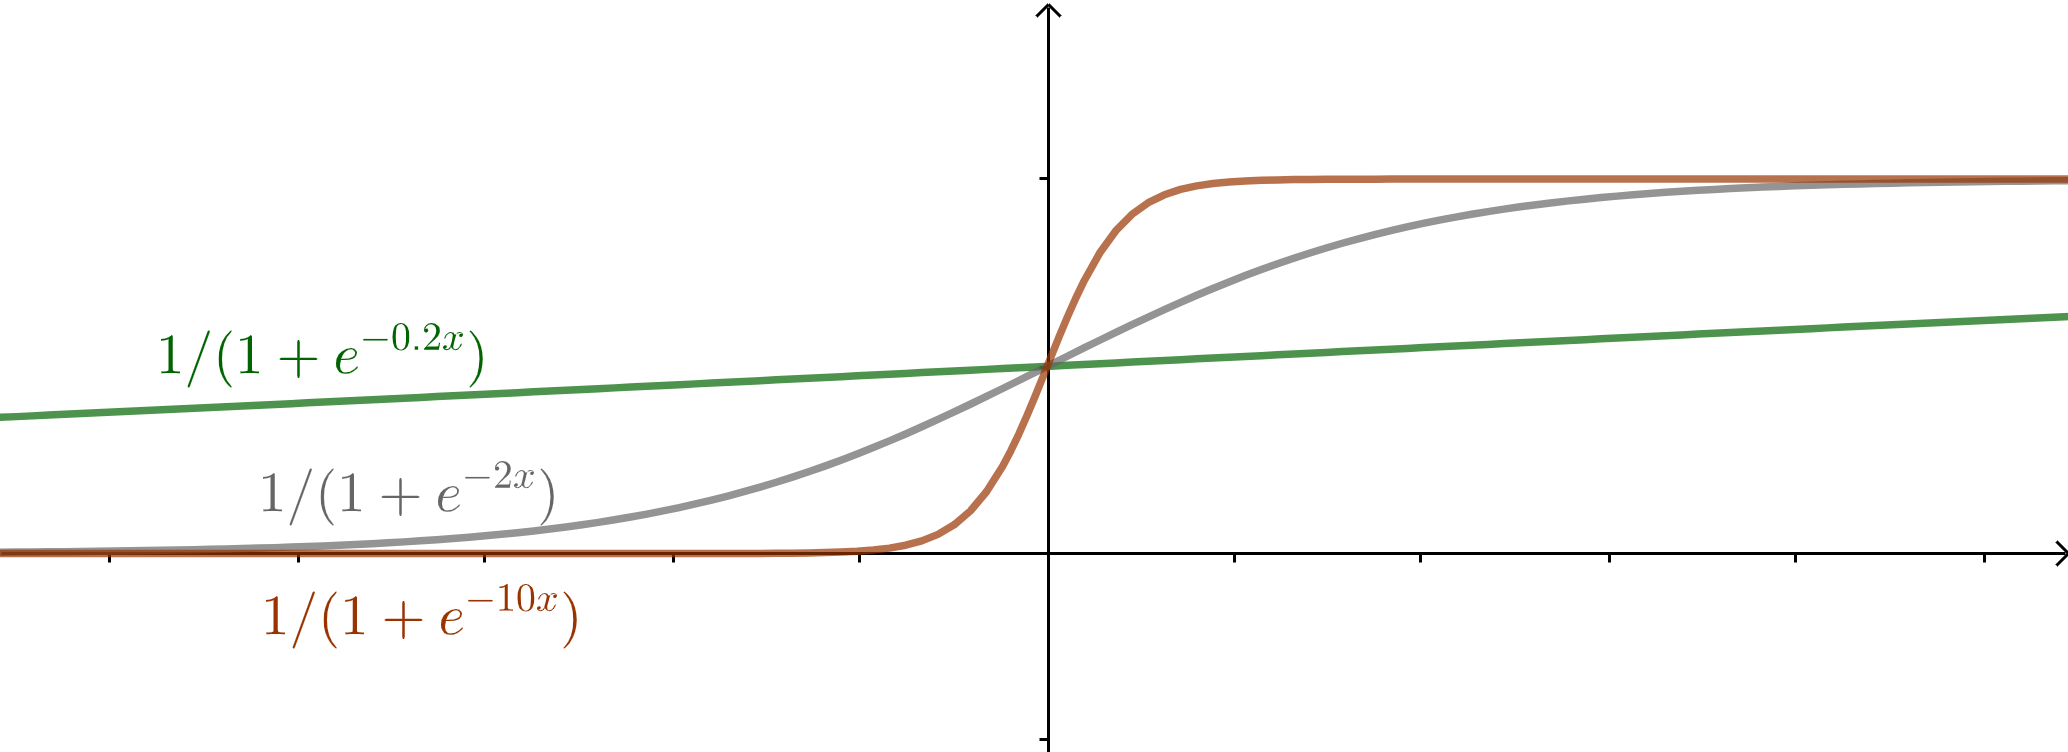
\includegraphics[width=9.5cm]{hinh_chuong2_convexfunc/chap2_sigmoid.png}
	\caption{Biểu diễn hàm sigmoid $\frac{1}{1 + e^{-w x}}$ với $w = 0,2; 2; 10$ trong không gian 2D.}
	\label{fig:sigmoid}	
\end{figure}

\subsection*{Hàm softmax}
Hàm \textit{softmax} $\mathbf{R}^n \rightarrow \mathbf{R}^C$ được dùng trong bài toán phân đa lớp  là log-concave
\begin{align*}
softmax(x)_i = \frac{e^{w_i^T x}}{\sum_{i=1}^C e^{w_i^T x}}, i=1,..., C
\end{align*}
Trong bài toán phân đa lớp dùng Bayes, $n$ là số đặc tính của điểm dữ liệu $x$ và $C$ là số lớp. 
Ví dụ trong ứng dụng nhận dạng chữ số viết tay dùng tập dữ liệu MNIST, khi đưa vào một hình chữ số viết tay $28\times 28 = 784$ pixel, giải thuật phân lớp sẽ dùng hàm softmax để ước lượng xác suất mà hình đó là chữ số nào. Đó là một vector có 10 thành phần là những xác suất mà hình đó là chữ số 0, 1,..., hay 9 ($C=10$). 
Nếu $softmax_2 = 0.91$ và 09 thành phần còn lại đều là 0.01 thì khả năng 91\% hình đó là chữ số 2.
Ngoài ra, softmax còn được dùng cho ngỏ ra của mạng reural nếu dùng mạng neural để phân đa lớp.

%\item Hàm phần bố chuẩn là log-concave:
%\begin{align*}
%f(x) = \frac{1}{\sqrt{(2\pi)^n det \Sigma}} exp(-\frac{1}{2}(x - \bar{x})^T \Sigma^{-1}(x - \bar{x}))
%\end{align*}
%\end{itemize}

%{Properties of log-concave functions}
%\begin{itemize}
%\item twice differentiable $f$ with convex domain is log-concave if and only if
%\begin{align*}
%f(x) \nabla^2 f(x) \preceq \nabla f(x) \nabla f(x)^T.
%\end{align*}
%\item product of log-concave functions is log-concave
%\item sum of log-concave functions is not always log-concave
%\item integration: if $f: \mathbb{R}^n \times \mathbb{R}^m \rightarrow \mathbb{R}$ is log-concave, then
%\begin{align*}
%g(x) = \int	f(x, y)dy 
%\end{align*}
%is log-concave

%
%\section{Bài tập}
%
%\subsection*{Bài tập về tập lồi}
%
%\begin{enumerate}
%\item Những tập nào sau là các đa diện:
%	\begin{enumerate}[a.]
%	\item 
%	$S = \{y_1 a_1 + y_2 a_2 | -1 \leq y_1, y_2 \leq 1 \}$, trong đó $a_1, a_2 \in \mathbf{R}^n$.
%	
%	\item 
%	$S = \{x \in \mathbf{R}^n | x \geq 0, 1^T x = 1, \sum_{i=1}^n x_i a_i = b_1, \sum_{i=1}^n x_i a^2_i = b_2\}$, trong đó $a_1,..., a_n, b_1, b_2 \in \mathbf{R}$.
%	\end{enumerate}
%
%\item
%
%
%\item 
%Hàm phối cảnh (perspective function) $f: \mathbf{R}^{n+1} \rightarrow \mathbf{R}^{n}$ là hàm số $f(x,t) = x/t$, với $x\in \mathbf{R}^n$ và $t \in \mathbf{R}, t >0$.
%Hàm này biến đổi một điểm (tức là một vector) trong không gian $\mathbf{R}^{n+1}$ chiều thành một điểm trong không gian $\mathbf{R}^{n}$ bằng cách bỏ thành phần cuối cùng và chia các thành phần trước đó cho thành phần cuối cùng.
%Trong không gian ba chiều, hàm này tương tự như thể hiện một vậy thể 3D trên môt mặt phẳng 2D.
%Trực quan thì hình ảnh của một vật lồi cũng là một hình lồi.
%
%Chứng minh nếu $C$ là tập lồi thì $f(C)$ cũng là tập lồi.
%
%\saveenum
%\end{enumerate}
%
%\subsection*{Bài tập về hàm lồi}
%\begin{enumerate}
%\resume
%\item Chứng minh mọi hàm norm là hàm lồi.
%\item
%\end{enumerate}

%\section{Ghi chú}
%Có nhiều nguồn tài liệu cho phép người học làm quen với ngôn ngữ Python, ví dụ \cite{pythonbook}.
%Các bài tập trong chương này được tham khảo từ các sách \cite{guenin, boyd}

\begin{thebibliography}{8}
\bibitem{boyd}
Boyd, Stephen, Stephen P. Boyd, and Lieven Vandenberghe. Convex optimization. Cambridge university press, 2004.

\bibitem{pythonbook}
Wentworth, Peter, Jeffrey Elkner, Allen B. Downey, and Chris Meyer. How to think like a computer scientist: Learning with Python 3. (2015).

\end{thebibliography}

\end{document}